\documentclass[a4paper,10pt]{jsarticle}
%\documentclass[a4paper,10pt]{jsbook}

\usepackage[dvipdfmx]{graphicx, color}
%\usepackage{folha}
\graphicspath{{image/}}

\usepackage{color}
\usepackage{array}
\usepackage{longtable}
\usepackage{alltt}
\usepackage{graphics}
\usepackage{vpp-nms}
%\usepackage{vpp}
\usepackage{makeidx}
\makeindex

\usepackage{colortbl}

\usepackage[dvipdfmx,bookmarks=true,bookmarksnumbered=true,colorlinks,plainpages=true]{hyperref}

%\AtBeginDvi{\special{pdf:tounicode 90ms-RKSJ-UCS2}}
\AtBeginDvi{\special{pdf:tounicode EUC-UCS2}}

\definecolor{covered}{rgb}{0,0,0}      %black
\definecolor{not-covered}{rgb}{1,0,0}  %red

\setcounter{secnumdepth}{6}
\makeatletter
\renewcommand{\paragraph}{\@startsection{paragraph}{4}{\z@}%
  {1.5\Cvs \@plus.5\Cdp \@minus.2\Cdp}%
  {.5\Cvs \@plus.3\Cdp}%
  {\reset@font\normalsize\bfseries}}
\makeatother

\renewcommand{\sf}{\sffamily \color{blue}}

\newcommand{\syou}{\texttt{<}}
\newcommand{\dai}{\texttt{>}}

%\include{Title}

%\pagestyle{empty}
\usepackage{fancyhdr}
\usepackage{lastpage} 
  \pagestyle{fancy} 
   \let\origtitle\title 
  \renewcommand{\title}[1]{\lfoot{#1}\origtitle{#1}}

  \rfoot{\today}
  \rhead{[\ \scshape\oldstylenums{\thepage}\ / %
      \scshape\oldstylenums{\pageref{LastPage}}\ ]}
  \cfoot{}


\begin{document}

% the title page
\title{エクスプレス予約システムの問題点を推測し、修正した仕様}
\author{佐原 伸\\\\
SCSK (株)\\
}
%\institute{\pgldk \and \chessnl}
\date{\mbox{}}
\maketitle

%\TaoReport{ガードコマンド・モデル}{\today}{タオベアーズ}{佐原伸}
%\setlength{\baselineskip}{12pt plus .1pt}
%\tolerance 10000
\tableofcontents
%\thispagestyle{empty} 

%\include{Abstract}
\section {発端}
鉄道会社Aの特急券予約システムで特急券を2枚予約し、
以下のような「事件」が起こったのが本モデルを書いた理由である。


以下のやりとりは、電話でのやりとりをかなり(主として用語を中心として)整理したものである。
実際には、例えば、鉄道会社Aサポートセンターの担当者は「カード」という言い方をするのだが、
それがクレジットカードの場合と、予約会員証の場合と、ICカードあるいは予約カードの場合があったので、
個々の用語の正確な名前と意味を調べるだけで
かなりの日数と時間を要した問答であった。

ICカードと予約カードは、結局、この問題とは直接は関係なかったので、この後、本稿に登場することはない。

\begin{itemize}
\item おサイフケータイ(鉄道会社B)で特急券予約システム(鉄道会社A)を使っていた
\item ロンロンViewカードが廃止になりアトレクラブViewカードに変更して下さいとの連絡があった
\item 予約できなかったので 鉄道会社Aサポートセンターに電話

	\begin{description}
	\item [客]「特急券を2枚予約しようとしたが、予約できなかったんですが?」
	\item [JR]「カードを変更したら、特急券予約システムを新規に契約して下さい。」
	\item [客]「新規にすると会費がかかるのでは?」
	\item [JR]「はい。」
	\item [客]「カード会社の都合で変更するのに、それはおかしいでしょう?」
	\item [JR]「では、無料にします。」
	\end{description}

\item 特急券に引換えできなかったので 鉄道会社Aサポートセンターに電話

	\begin{description}
	\item [客]「新しい予約はできたんですが、クレジットカード変更前に予約した特急券に引換えようとしたらできないのですが?」
	\item [JR]「予約会員証で引換できるようになったので、それで引換えて下さい。
			暗証番号はクレジットカードのものを使って下さい。」
	\end{description}

\item T駅での問答

	\begin{description}
	\item [客]「会員証で特急券に引換えできないのですが?」
	\item [JR]「会員証で引換えできないですねー。おかしいな。クレジットカードでやってみましょう。駄目ですねー。」
	\item [客]「古いクレジットカードでは駄目ですか?」
	\item [JR]「あ、できましたね。はい、切符です。」
	\end{description}

\end{itemize} 


\section {モデル化の範囲}
この問題で登場する用語には以下がある。

\begin{itemize}
\item 鉄道会社A、鉄道会社B
\item おサイフケータイ
\item 特急券予約システム
\item 予約会員証、ICカード、予約カード
\item クレジットカード
	\begin{itemize}
	\item ロンロンViewカード、アトレクラブViewカード
	\end{itemize} 
\item 特急券
\end{itemize} 

「鉄道会社B」「ICカード」「予約カード」は、モデルを単純化するため対象としなかった。

「鉄道会社A」の「特急券予約システム」システムのうち、
以下の機能だけをVDM++\cite{SCSK2012PP}で要求仕様としてモデル化し、
問題点を明確化することにした。

\begin{itemize}
\item 予約する
\item 特急券を得る
\item クレジットカードを切り替える
\end{itemize} 

従って、モデル化する範囲に登場するpublicな用語は以下だけである。
\begin{itemize}
\item おサイフケータイ
\item 特急券予約システムシステム
\item 特急券予約システム
\item 予約会員証
\item クレジットカード
\item 特急券
\end{itemize} 





	
\include{ReservationSysytem.vpp}	
\include{Common.vpp}
\include{ReservationDomain.vpp}
\include{ReservationDomainData.vpp}
\include{ExpressReservatiopn.vpp}
\include{Contract.vpp}
\include{Card.vpp}
\include{CredirCard.vpp}
\include{CustomerCard.vpp}
\include{SUICA.vpp}
\include{MyTest.vpp}
\include{MyTestCase.vpp}
\subsubsection{まとめ}
\paragraph{問題は何だったのか?}
結局、問題は何だったのかといえば、
特急券予約システムのクレジットカードによる決済のモデルが考慮不足だったということになる。

まず、おサイフケータイのクレジットカードを変更すると、
特急券予約システムを新規に契約せねばならず、
予約会員証も新規に作成しなければならない。

しかし、変更前の予約を行った古いクレジットカードは、
その予約の特急券を受け取るときに必要になる。
何故なら、クラス図\ref{fig:ExpressReservationClassDiagram}で見るように、
個々の予約を表す特急券予約システムからクレジットカードにリンクが設定されているからである。

\begin{figure}[h]
	\centering
	{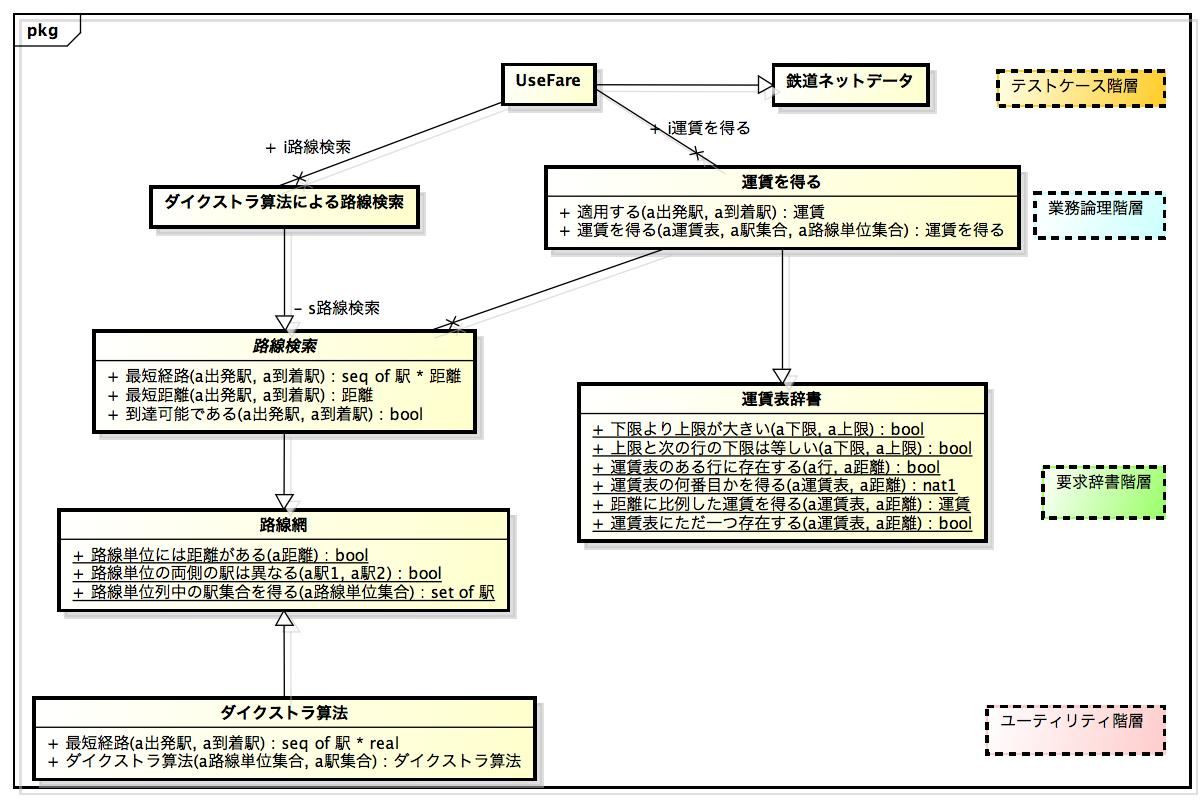
\includegraphics[width=55zw, keepaspectratio]{./image/ClassDiagram.jpg}}
	\caption{クラス図(特急券予約システム)}
	\label{fig:ExpressReservationClassDiagram}
	\index{くらすすとっきゅうけんよやくしすてむ@クラス図(特急券予約システム)}
\end{figure}

このような構造でも、変更後にすべての特急券予約システムからクレジットカードへのリンクを
新しいクレジットカードに変更していれば問題はないはずだが、
恐らく、変更に掛かる効率を理由に、古いクレジットカードとリンクしたままになっているのであろう。
設計上の理由で、ユーザーに迷惑を掛ける仕様となっている訳である。

さらに、モデルに問題があった。
予約会員証は新規に作るのが普通であるが、
クレジットカード会社の都合による変更のため、
新規に契約する費用は無料となった。
そのため、予約会員証は古いものを使用することになった。
契約は新規だが、予約会員証は古く、
そしてクラス図\ref{fig:ExpressReservationClassDiagram}から分かるように、
予約会員証からリンクしているクレジットカードは、
変更前の古いものであるという訳である。

これではまずいと思って、鉄道会社Aの係員がリンクされているクレジットカードを新しいものにしたようである。
その結果、変更前の特急券予約システムを予約会員証で特急券を得ることができなかった。


\paragraph{本来どうすべきだったのか?}
本来、特急券予約システムは契約\footnote{口座と言ってもよいが、本モデルでは契約という名前にした}
とリンクが設定されているべきであり、
契約がクレジットカードとリンクしているべきである。

予約会員証も契約を介してクレジットカードを参照できるようにすべきである。

このようにしておけば、契約に変更があっても、古い特急券予約システムは新しい契約を介して、新しいクレジットカードにアクセスでき、
同じく予約会員証も新しいクレジットカードにアクセスできる。

本来どうすべきだったのかを検証するVDM++モデルは、1日で記述および検証ができた。

詳細は、「特急券予約システムシステムの問題点を推測し、修正した仕様」を参照のこと。


\paragraph{統計情報}
注釈抜きのVDM++ソース行数は、492行、
モデル作成工数は約1日、発表用の資料作成とVDM++モデルの読みやすさのための整形・清書に約2日かかった。

なお、上記モデルの作成工数は、筆者が問題を解決するために消費した工数より少ない。

%\begin{thebibliography}{9}
\section{参考文献等}
VDM++\cite{CSK2007PP}は、
1970年代中頃にIBMウィーン研究所で開発されたVDM-SL\cite{CSK2007SL}を拡張し、
さらにオブジェクト指向拡張したオープンソース
\footnote{使用に際しては、(株)CSKシステムズとの契約締結が必要になる。}の形式仕様記述言語である。
\bibliographystyle{jplain}
%\bibliography{/Users/sahara/svnw/sahara}
\bibliography{/Users/sahara/bib/saharaUTF8}
%\bibliography{/Users/ssahara/svnwork/sahara}

%\end{thebibliography}

%\newpage
%\addcontentsline{toc}{section}{Index}
\printindex

\end{document}
